\section{RMHD Models of PWN}
\subsection{Simulating the plasma flow         (SK, OP, AL, BO, EA)}
\subsection{Radiative predictions, from particle transport models      (OP, AL, EA)}
\subsection{Gamma-ray binaries: pulsar winds interacting with a massive companion}
\subsubsection{Introduction}
The last decade revealed a new  a new group of gamma ray emitters, composed of a fast-rotating pulsar and a massive star. The emission, which peaks in the MeV band, arises from the shocked region between the stellar wind and the pulsar wind. Particle acceleration at the relativistic shock creates emission up to several TeV, the highest emission observed for binary systems. Fig.~\ref{fig:gamma_binary} presents a schematic view of interaction region. A handful of these systems have been discovered so far: PSR B1259-63 \citep{2005A&A...442....1A}, LS 5039 \citep{2005Sci...309..746A} ,LSI +61$^o$ 303 \citep{2006Sci...312.1771A}, HESS J0632+057\citep{2011ApJ...737L..11B}, 1FGL J1018.6-5856 \citep{2010ApJS..188..405A}, and more recently HESS J1832-093 \citep{2016MNRAS.457.1753E}. While pulsed emission has been observed for PSR B1259 (thanks to its wide orbit), and LSI+ 61$^o$ 303 has shown magnetar type flares \citet{ATEL}, the nature of the compact object is not firmly established in the other systems. However, given the very similar emission patterns, the colliding wind scenario is now firmly established. As such, the major aspects of the colliding wind structure and the high-energy emission mechanisms have been assessed, and while many questions remain, the study of  gamma-ray binaries has matured enough to become a new window on pulsar wind physics.  These systems provide a unique opportunity to study otherwise very elusive pulsar winds. The binary interaction typically takes place around a fraction of  AU from the pulsar (or about $10^4$ times the light cylinder), about 5 orders of magnitude closer than for pulsars interacting with the ISM.  Modeling strongly benefits from information provided by orbital variability and  the well constrained environment created by the companion star, both in terms of density and photons fields (at least compared to a typical region of the ISM).  While an excellent review can be found in \citet{2013A&ARv..21...64D}, this section provides some updates and focuses on how to determine the pulsar wind properties from the emission of gamma-ray binaries.


\begin{figure}[h]  
\centering
  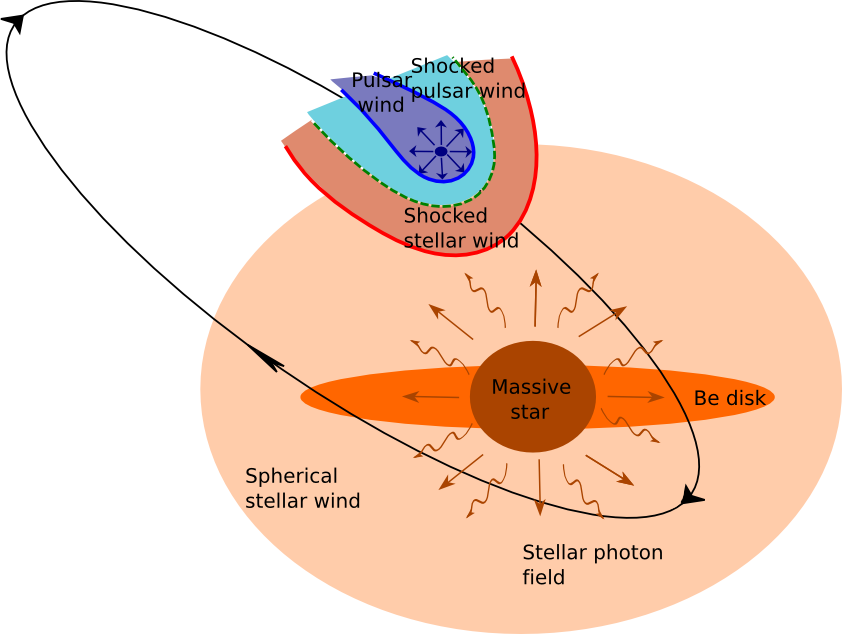
\includegraphics[trim=2cm 1cm 2cm .5cm, clip,width=.65\textwidth]{gamma_binary}
\caption{Schematic view of a gamma-ray binary. The pulsar wind interacts with the stellar wind,  photon field and circumstellar disk if the companion is a Be star.}
\label{fig:gamma_binary}
\end{figure}




\subsubsection {$\gamma$-ray binaries : puzzling observations}
While most of the energy is emitted in MeV photons (hence the name), gamma-ray binaries emit all the way from radio to a few TeV. Fig.~\ref{fig:obs} shows the high energy spectral energy distribution of PSR B1259-63 with emission resulting from the electrons accelerated at the shocks between the winds. Acceleration at the relativistic shock produces synchrotron emission (up to a few GeV) and Inverse Compton emission on seed photons of the massive star (up to a few TeV).   


In theses systems, most of the emission (with the exception of the low frequency radio band \citep{2015MNRAS.451...59M}) shows orbital variability. The right panel of  Fig.~\ref{fig:obs} shows lightcurves of LS 5039, a binary with a 3.9 day period:  X-ray and TeV emission show similar orbital variability, in opposition with the variability observed with $Fermi/LAT$.  The MeV emission in LS 5039, with an exponential cutoff at a few GeV before the harder but fainter TeV emission cannot be reconciled while assuming emission from a single population \citep{2008A&A...477..691D}. The different origin of the GeV and TeV emission is also suggested by the absence of emission below 200 GeV  in HESS J0632+057  \citep{2016arXiv160108216M} and around periastron in PSR B1259-63, while both show strong TeV emission.  

 LSI+61303 shows additional variability on superorbital timescales \citep{2012ApJ...747L..29C}, attributed to long-term variations in the Be disk surrounding the companion star \citep{2015A&A...575L...6P}. Interactions with the Be disk are likely responsible for the suborbital optical line variability in HESS J0632+057 \citep{2015ApJ...804L..32M}. 

In PSR B1259-63, which has a 3.4 year period, X-rays, TeV and radio flares are observed about 15 days before and after periastron. Optical spectroscopy indicates these flares are consistent with the disruption of the Be disk ask the pulsar crosses it \citep{2016MNRAS.455.3674V}.  About 60 days after periastron, $Fermi/LAT$ detects strong emission with no counterpart at any other wavelength \citep{2011ApJ...736L..11A}.  This flare, which contains almost all the spindown power of the pulsar,  has been confirmed at the 2014 periastron passage \citep{2015ApJ...811...68C} with a similar flux level and spectral shape but slightly different temporal evolution.  


Extended radio emission traces the contours of the shocked region \citep{2006smqw.confE..52D,2011ApJ...732L..10M}. Extended X-ray emission has also been found for most (if not all) of these systems but its origin remains unclear  \citep{2014AN....335..301K}. 


\begin{figure}
  \centering
  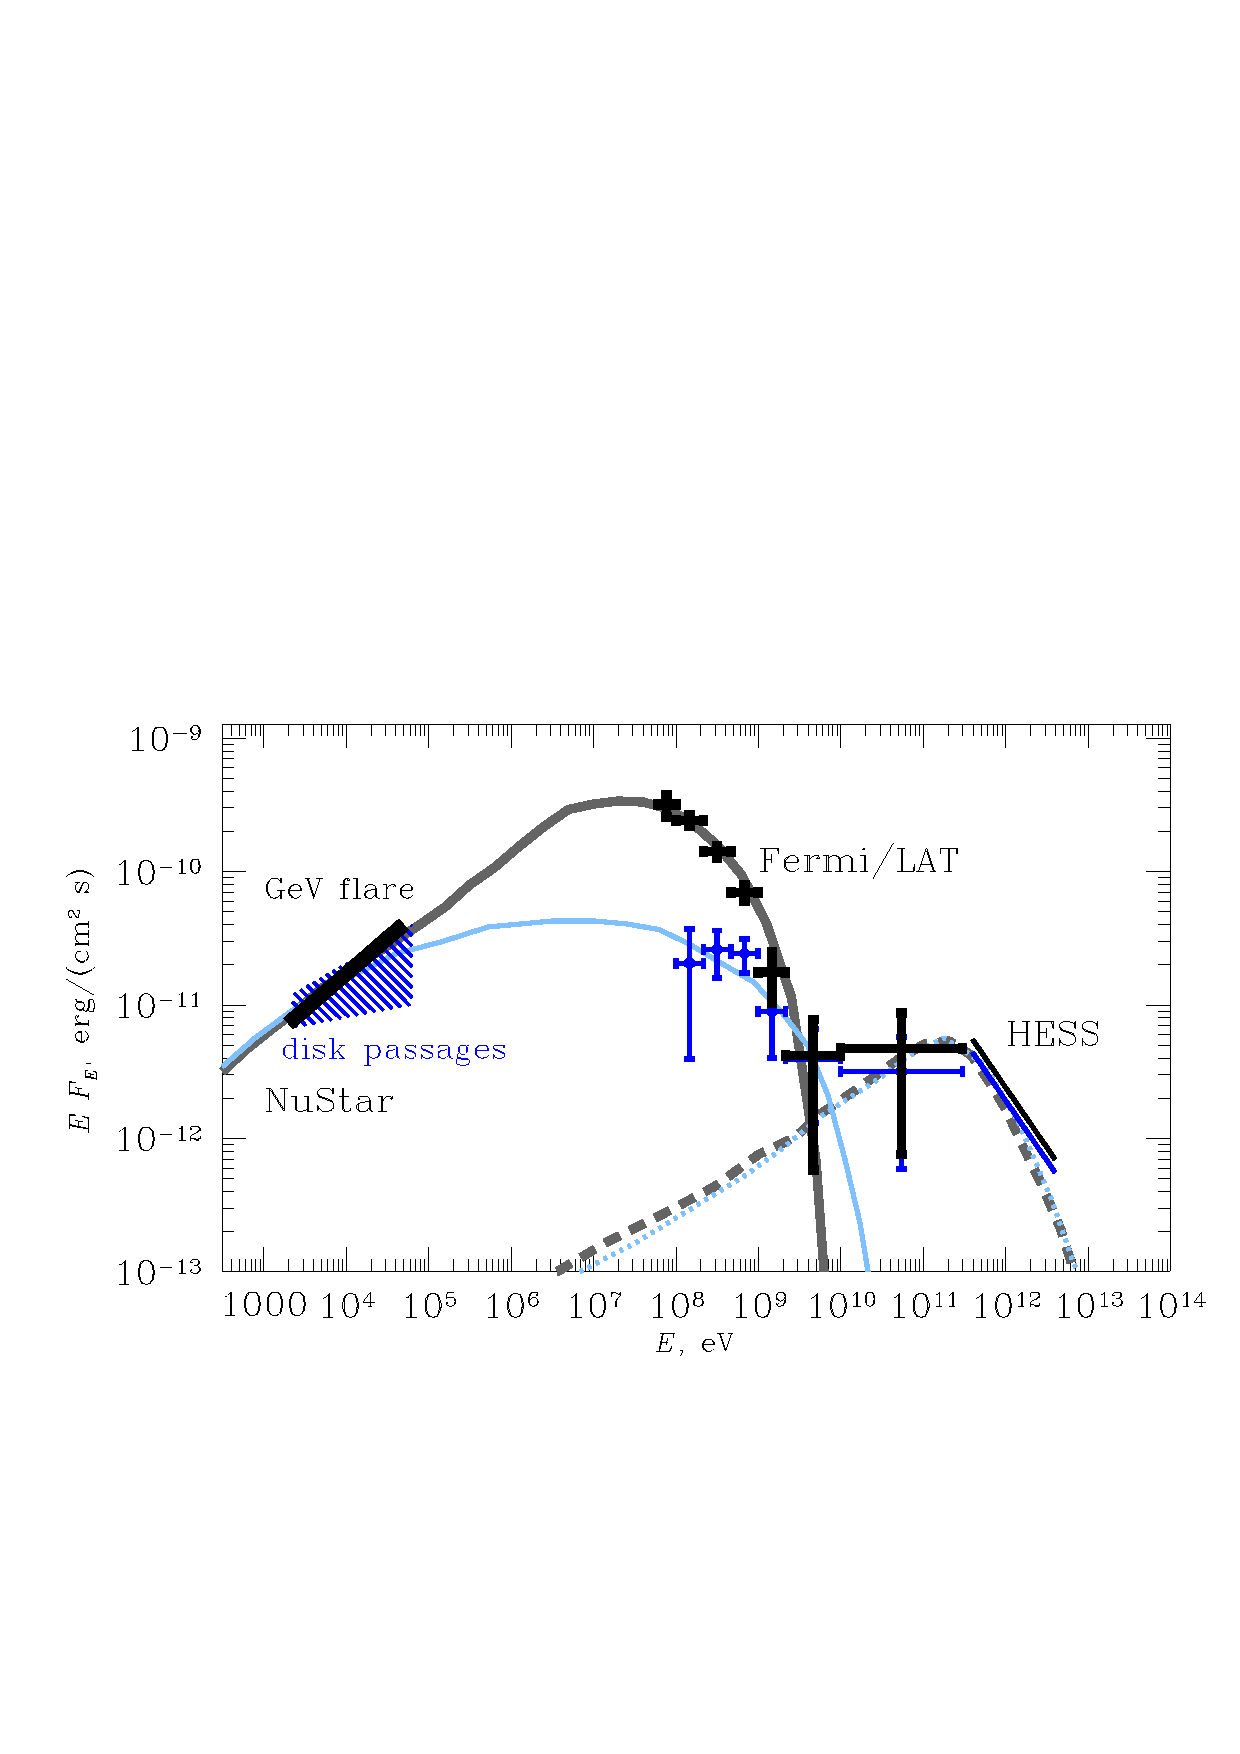
\includegraphics[width = .45\textwidth ]{PSRB_spectrum_broadband}
\includegraphics[width=.4\textwidth]{ls5039_light}
  \caption{Left : Spectral energy distribution of PSR B1259-63, during the disk passages (blue) and flares (grey) (from \citet{2015MNRAS.454.1358C} ). Right : X-ray, GeV and TeV modulation for LS 5039. (Adapted from \citet{2009ApJ...697L...1K,2009ApJ...706L..56A} and \citet{2006A&A...460..743A} .)}
  \label{fig:obs}
\end{figure}


\section { Ingredients for successful models}


The wide variety of observational constraints is both a challenge an a tremendous opportunity to understand these systems.  Until recently, studies have either focussed on sophisticated one-zone emission models or aimed at reproducing the hydrodynamical  structure of the colliding wind region, with litte connexion to the non-thermal emission. While both approaches have had been fruitful, they have not been able to consistently reproduce the  orbital variability and spectral features from radio up to TeV.   The next sections describe both approaches and how they can be combined to yield a better understanding of pulsar wind physics.

The first ingredients are the non-thermal emission processes, dominated by leptonic processes \citep{2006A&A...456..801D}, causing a synchrotron bump and inverse Compton bump.  Models have included refined  representations of the ambient photon field, including self-Compton the on the nebula  \citep{2010A&A...519A..81C} and the infrared photons of the  Be disk when present  \citep{2012MNRAS.426.3135V}. Reproducing the TeV lightcurve of LS 5039 requieres anisotropic inverse Compton emission  \citep{2008A&A...477..691D} as an extended emission region. The latter is necessary to prevent complete absorption by pair production at  superior conjunction in LS 5039 (when the compact object is behind the massive stars).  Inverse-Compton pair cascades could extend the emission region \citep{2006MNRAS.371.1737B,2010A&A...519A..81C}. Or, the  emission could also result from one or more  distant emission regions \citep{2013A&A...551A..17Z}.  Similarly, the presence the absence of occultation features in the X-ray lightcurves suggests an extended emission region \citep{2007A&A...473..545B,2011MNRAS.411..193S}.  As the emission originates from the relativistic shocked pulsar wind, Doppler boosting is also at work at inferior conjunction (when the pulsar wind points toward the observer) and explains some of the GeV modulations \citep{2010A&A...516A..18D}. 

%Inverse-Compton pair cascades could extend the emission region \citep{2006MNRAS.371.1737B,2010A&A...519A..81C}


 Single zone models have so far failed to consistently reproduce the full variability of the systems, even when cascase emission is allowed. The exponential cutoff around a few GeV is hard to reconcile with the hard TeV emission. A single particle distribution with IC, synchrotron  and adiabatic  cooling fails to reproduce  this spectral feature \citep{2008MNRAS.383..467K, 2013A&A...551A..17Z}.   The presence of an additional emission component has been suggested. While the GeV emission  is analogous to  pulsar magnetospheric emission observed by $Fermi$, it's orbital variations are hard to explain \citep{2012ApJ...749...54H}.   The emission of the unshocked pulsar wind \citep{2007MNRAS.380..320K}   has been considered but is insufficient \citep{2008APh....30..239S}.  A shocked mono-energetic  component have also been considered \citep{2013A&A...557A.127D}.  An alternate path is the presence of a different acceleration region, with different properties in terms of magnetic field, photon field and velocity structure \citep{2013A&A...551A..17Z}.

Over the years, it has become clearer that the only path towards fully understanding the emission in gamma-ray binaries would require an elaborate model for the geometry of the system, coupled with a refined model for the non-thermal emission. 

The flow dynamics in gamma-ray binaries are dominated by the double shock structure. It  shares many similarities with colliding stellar winds, which have been studied for decades. Simulations \citep{2009MNRAS.396.1743P,2011MNRAS.418.2618L} show strong instabilities which may  yield mixing in the winds \citep{2010MNRAS.403.1873Z}  and affect spiral structure expected at large scales \citep{2012A&A...546A..60L,2012A&A...544A..59B}.  

However, the relativistic nature of the pulsar wind affects the structure of the interaction region. Relativistic hydrodynamics yield more complex shock patterns, where parallel velocities (to the shock normal) play a role. Multidimensional simulations in the  ultrarelativistic regime of pulsar winds (Lorentz factor $\simeq 10^3-10^5$) are far beyond current computational and numerical capabilities. Some rescaling may be necessary even when focusing on the shocked winds,which have $\Gamma\lesssim 10$ close to the pulsar.  Simulations suggest a narrower opening angle for the pulsar wind \citep{2013A&A...560A..79L}, and a reacceleration of the pulsar wind up to its initial velocity \citep{2008MNRAS.387...63B}. Keeping in mind these intrinsic difficulties, relativistic simulations are crucial in order to determine Doppler boosting, which is a key ingredient to orbital modulation and maybe the GeV flares in PSR B1259 \citep{2012ApJ...753..127K}. Simulations suggest the presence of a back shock behind the pulsar, which can provide an additional site for particle acceleration, further away from the binary. They also indicate the presence of a large scale bubble as both winds interact with the ISM (verifier).





\begin{figure}[h]
  \centering
  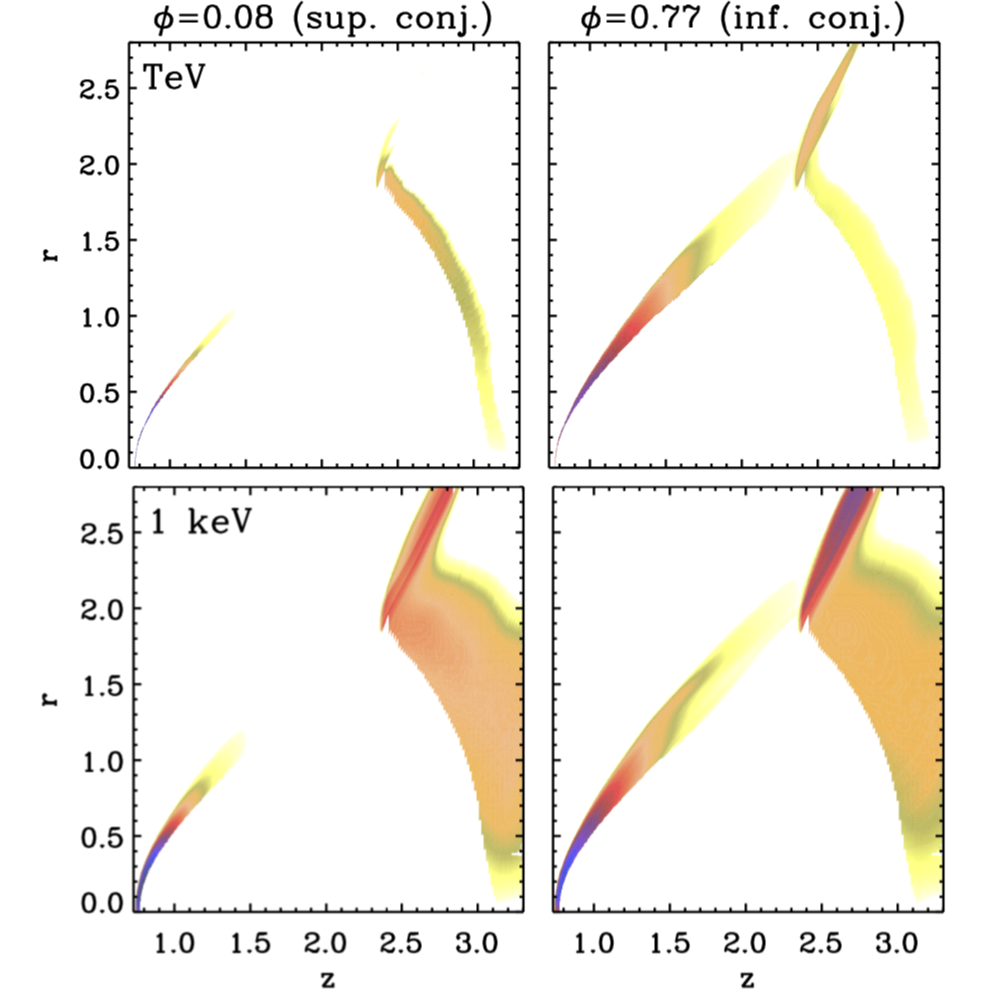
\includegraphics[width = .33\textwidth ]{emission_map}
  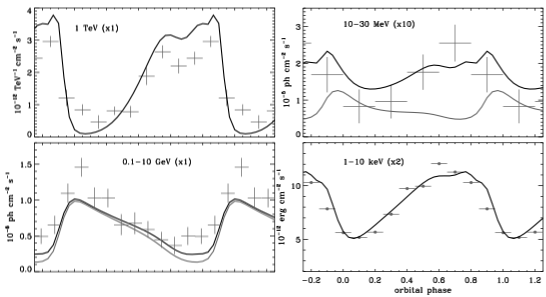
\includegraphics[width = .63\textwidth ]{all_curves}
  \caption{Left: TeV and X-ray emission maps for LS 5039 at superior and inferior conjunctions. Right: Simulations lightcurves for LS 5039 with a powerlaw particle distribution (black) and an additional mono-energetic component (grey). Images taken from \cite{2015A&A...581A..27D}.}
  \label{fig:LS5039}
\end{figure}

\citet{2015A&A...581A..27D} developed the first high energy emission model based on a fully three-dimensional relativistic simulations of LS 5039.  As explained in section \ref{sec:method}, the non-thermal emission is determined during post-processing, with a particle distribution injected at the relativistic shock and followed along the streamlines in the shocked pulsar wind. The model self-consistently represents adiabatic, inverse Compton and synchrotron cooling. The resulting emission takes into account pair creation, anisotropic Inverse Compton and directly benefits from the simulation to model Doopler boosting.  Fig. ~\ref{fig:LS5039} shows the resulting emission maps and lightcurves.  Comparison with observations suggested a strongly magnetized, rather slow pulsar wind ($\Gamma\simeq 10^3, \sigma \simeq 1$). While small discrepancies exist with observations, and radio emission won't be modeled properly without taking into account the magnentic field structure, the clear success of the combination of relativistic hydrodynamics with refined emission models shows the path forward in this field.



\subsection{The wisps as probes of  particle acceleration sites ? (BO)}
